%%
%% This is file `sample-sigplan.tex',
%% generated with the docstrip utility.
%%
%% The original source files were:
%%
%% samples.dtx  (with options: `sigplan')
%% 
%% IMPORTANT NOTICE:
%% 
%% For the copyright see the source file.
%% 
%% Any modified versions of this file must be renamed
%% with new filenames distinct from sample-sigplan.tex.
%% 
%% For distribution of the original source see the terms
%% for copying and modification in the file samples.dtx.
%% 
%% This generated file may be distributed as long as the
%% original source files, as listed above, are part of the
%% same distribution. (The sources need not necessarily be
%% in the same archive or directory.)
%%
%% The first command in your LaTeX source must be the \documentclass command.
\DocumentMetadata{
  lang=en,
  pdfversion=2.0,
  %pdfstandard=ua-2,
  %testphase={phase-III,firstaid,math,title}
  tagging=on,
  testphase={phase-III,firstaid,math,title}
  %tagging-setup={math/setup=mathml-SE}
}
\documentclass[sigplan,screen,nonacm]{acmart-tagged}
\usepackage{color}
\setlength {\marginparwidth }{2cm}
\usepackage[colorinlistoftodos]{todonotes}
\usepackage[
    type={CC},
    modifier={by-nc-sa},
    version={4.0},
]{doclicense}
%% NOTE that a single column version is required for 
%% submission and peer review. This can be done by changing
%% the \doucmentclass[...]{acmart} in this template to 
%% \documentclass[manuscript,screen,review]{acmart}
%% 
%% To ensure 100% compatibility, please check the white list of
%% approved LaTeX packages to be used with the Master Article Template at
%% https://www.acm.org/publications/taps/whitelist-of-latex-packages 
%% before creating your document. The white list page provides 
%% information on how to submit additional LaTeX packages for 
%% review and adoption.
%% Fonts used in the template cannot be substituted; margin 
%% adjustments are not allowed.
%%
%% \BibTeX command to typeset BibTeX logo in the docs
\AtBeginDocument{%
  \providecommand\BibTeX{{%
    \normalfont B\kern-0.5em{\scshape i\kern-0.25em b}\kern-0.8em\TeX}}}


%%
%% end of the preamble, start of the body of the document source.
\begin{document}

\title{Challenges of Optical Character Recognition}
\author{Orville ``El'' Anderson}
\email{and10393@umn.edu}
\affiliation{
  \institution{Division of Science and Mathematics 
	\\
        University of Minnesota, Morris
	}
  \city{Morris}
  \state{Minnesota}
  \country{USA}
  \postcode{56267}
}

%%
%% The abstract is a short summary of the work to be presented in the
%% article.
\begin{abstract}
Optical Character Recognition (OCR) is technology used to extract text from images. 
[this technology has a variety of uses and is very cool]
OCR has three main categories of challenges that reduce accuracy when applied to scanned documents, stemming from page layouts, the alphabet used, and visual noise.
By intentionally expanding the documents used to train modern OCR models, we can increase the range of capabilities of this technology. 
This paper looks at some of the ways that OCR models have adapted to address these challenges, and looks at some examples of datasets which are made to cover some of these document variations.
% This paper looks at the Tesseract, Amazon Textract, and Google Document AI models, as applied to English and Arabic documents.
\end{abstract}

\doclicenseThis

%%
%% Keywords. The author(s) should pick words that accurately describe
%% the work being presented. Separate the keywords with commas.
\keywords{optical character recognition, scanned documents, layout, languages, visual noise, datasets}


%%
%% This command processes the author and affiliation and title
%% information and builds the first part of the formatted document.
\maketitle

\section{Introduction}
\label{sec:introduction}

Over time, American institutions have accumulated a tremendous amount of scanned documents. 
In April of 2024, the Department of Justice updated the Americans with Disabilities Act to include access to digital content such as scanned documents. 
Among other requirements, all scanned documents made publicly accessible by state and local governments must now be usable by a screen reader.

When a document is scanned, it becomes an image and looses all record of the content found on the original document. The first step to make a scanned document screen-readable is to recognize the text lost when the document was scanned. This process can be done manually, but that isn't well suited for large numbers of documents. Instead we look to Optical Character Recognition (OCR), a technology made to extract text from images.

The background section of this paper covers the three main steps in OCR. The Challenges section looks at how layout, alphabet, and visual noise impact OCR output accuracy. The Results section looks at two examples of datasets made to address these challenges and looks at how the OCR model Tesseract, has adapted to address some of these challenges. The Conclusion section discusses the importance of specialized datasets and increasing OCR accuracy in these cases.

\section{Background}
\label{sec:background}
The process of OCR starts with an existing scanned document. These documents can come in many file types, some common ones are .tiff, .pdf, and .jpg.
% The first step in using OCR on a document is to acquire an image of the document. This can be done using a camera or a scanner. These images can be saved as a variety of formats, such as a .pdf, .jpg, or .png. 
This file is then input to an OCR model, where the model will go through the three stages of OCR.\ref{fig:stages} The model will then return the text identified in the document as plain text, sometimes with meta-information. \footnote{Modern OCR models can use this meta-information and text to construct new output formats.}

\begin{figure*}
\centering
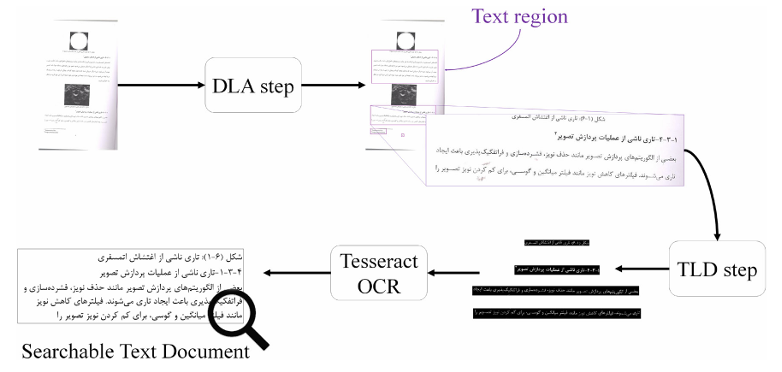
\includegraphics[width=\textwidth]{stages.png}
\caption{Stages of OCR}
\Description{Some description}
\label{fig:stages}
\end{figure*}

As seen in figure \ref{fig:stages}, the first stage of OCR is Document Layout Analysis which breaks down the page into sections of text. The second stage is Text Line Detection, which then further breaks down those sections into individual lines of text, or into individual words. The final stage is Classification and Recognition which identifies the text and outputs it as a searchable text document.

\subsection{Document Layout Analysis}
\label{DLA}
The first step in OCR is Document Layout Analysis (DLA), and is a general pre-processing step. The purpose is to identify what part of the image is text and what is not. This effectively draws a box around each paragraph and table on the page.
% This step addresses some of the complexity introduced when the image was made. This step can include rotating the full image and cropping out borders.
This step frequently outputs the result as a binary image, where each pixel is marked as a text or non-text pixel, to reduce computation costs.

An important step of DLA is preserving the reading order of the document. Without this step, OCR models are effectively limited to simple single-column text inputs.

\subsection{Text Line Detection}
\label{TLD}
Text Line Detection (TLD) is the second step in OCR. TLD takes the blocks of text from the previous step and further breaks them down, into lines, words, and then individual characters. The output of this step is each identified character in its own defined box of pixels.

A common technique used in this step includes rotating the individual lines of text to create a baseline. This can be seen in figure \ref{fig:stages} where the text entering the TLD step is at an angle, but the output is rotated so each line is horizontal
% Two methods employed by Fateh et al\citep{Fateh:2024} used font size and correcting line rotation, to improve overall accuracy.
% After the individual characters have been identified, we go through and look at each of the boxes we have drawn around the characters and mark which pixels we think are text and which are not.

\subsection{Recognition}
\label{Recognition}
The final step in the OCR process is referred to as Classification or Recognition. 
This step takes the boxes of individual characters from the last step and tries to identify the character inside of them.

% [One key thing to understand is that] An OCR model is only able to classify a character as something it has seen before.  

One common technique to identify an unknown character uses a process known as matrix matching. 
In this process, the unknown character is compared to an existing collection of known characters, and the character with the most similarity is chosen. \cite{Thorat:2022}
Another popular technique, called feature extraction uses measurements like character height, width and presence of loops to identify a character.
There are a lot of variations in classification techniques, but the key thing to note here is that all methods use some sort of reference material as a basis to classify characters. \cite{Thorat:2022}
The output of this recognition step is inherently limited to characters the model has been trained on.
% There are variations in classification techniques, including a subsection of OCR called Intelligent Character Recognition which uses machine learning, but all methods use some sort of training or reference material to classify.

%\subsection{Post-Processing}
%\label{sec:Post-Processing}
%
%Post-processing is an optional, but very common step for OCR, consisting of spellcheck and formatting. Running spellcheck on the output generally improves accuracy, but will write over spellings from the source document(misspellings and unconventional spellings included.) The additional formatting step is used to return the document to a human readable form. Some OCR will place the output directly over the input image, some will make webpages with the output and some will --.

%\subsection{Comparison}
%\label{comparison}
%
%The main considerations when judging OCR models are accuracy and speed.\cite{Avyodri:2022} 
%
%%[Speed is measured with a timer]
%
%A popular way to measure the accuracy of OCR output is to run the OCR program on a document where the page content is know. The OCR output is then compared to the known content and is measured by [the formula below], where x is a unit of measurement, like a line, word, or character.
%\[
%\dfrac{\sum\limits_{i=1}^\text{num of pages}\text{number of x correctly indentified}}{\sum\limits_{i=1}^\text{num of pages}\text{number of x on the page}}
%\]
%
%% \cite{Hegghamer:2022} this paper makes a destinction between word accuracy and character accuracy saying that "----"

\section{Challenges}
\label{sec:body}
There are three main categories of issues that decrease accuracy in the OCR process. Each of these challenges tie back to the key concept that OCR models work best when applied to what they were made to recognize.

\subsection{Layout}
\label{Layout}
Documents come in many different layouts. Images, figures, number of columns, and similar aspects add a layer of complexity to documents. In the Document Layout Analysis step and when the model outputs the final result, to be accurate, the model must have some method to understand the reading order. 
% In the Document Layout Analysis step of OCR the model must know which parts of the page to ignore, but also to know what order the sections of text should go in.
A paper formatted with two columns, such as this, is meant to be read left column, then right column. Unless otherwise instructed, an OCR model will take the first line from each column and treat them as one line. 
% While understanding paragraph breaks and readign order is generally intuitive, this is something that must be intentionally taken into account when training OCR.

Some OCR models are intentionally made to only handle one layout, such as a specific tax form or a job application for a specific company. A specialized OCR model, when applied to the layout it is made for, yields higher accuracy. This increase in accuracy is not applicable to layout beyond the intended one, and is generally not combined with other layout-specific models.

One related challenge to OCR accuracy is curved lines of text. As seen in figure \ref{fig:stages}, the text on the source document was angled. In this figure you can also see that the DLA and TLD stages use rectangles to section off portions of text. By intentionally rotating the lines of text, the boxes are a tighter fit to the text, creating more consistency between the characters and increasing accuracy. \cite{Fateh:2024}

\begin{figure}
  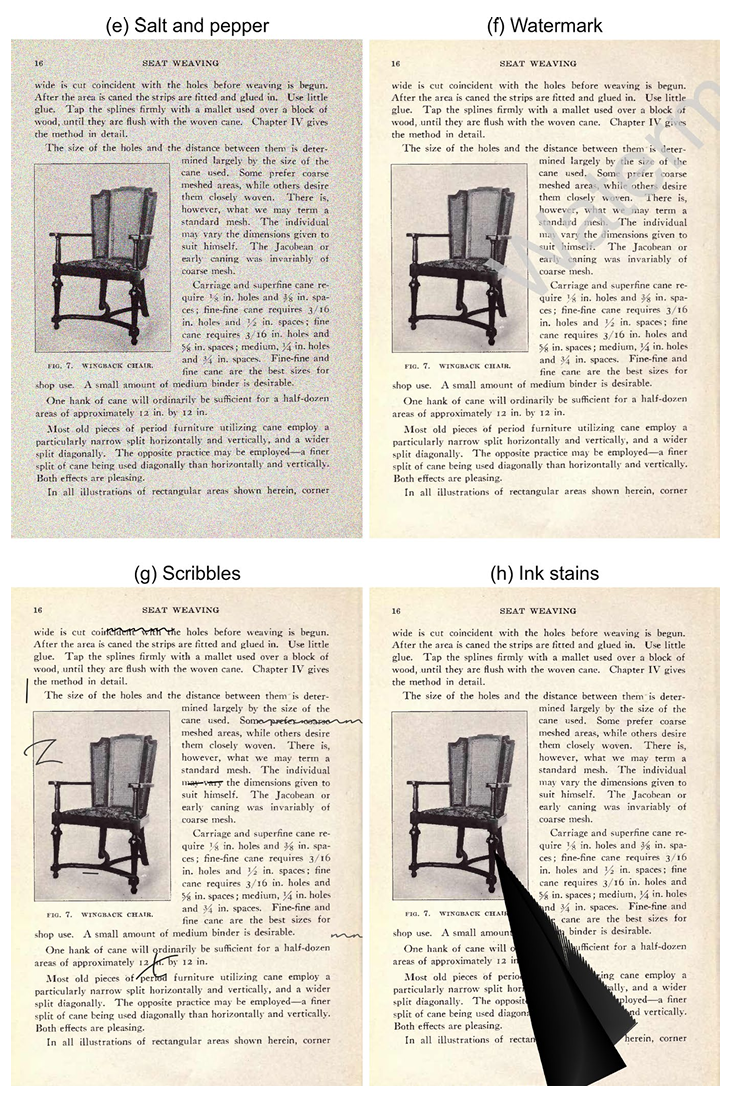
\includegraphics[width=\linewidth]{noise.png}
  \caption{Examples of visual noise from Hegghamer:2022, Salt and Pepper, Watermark, Scribbles, and Ink Stains}
  \label{fig:noise}
\end{figure}

\subsection{Visual Noise}
\label{Noise}

% There's so many ways to scan a document badly. \cite{Hegghamer:2022}
One big factor in the accuracy of OCR is the quality of the initial image. Marks on the physical document, book spines, and low image resolution all add additional complexity to the process. Marks on the page can both obscure letters, and can also be recognized as letters.

\subsection{Alphabet}
\label{Alphabet}
The most commonly used writing systems, by users, are the Latin alphabet, Chinese characters, then the Arabic alphabet.\cite{Vaughan:2025} \footnote{Arabic is actually an abjad, not a "true alphabet" because of how it treats vowels.}
The majority of OCR models are trained to recognize characters from the Latin alphabet.
As mentioned in section 2.4 Comparison, OCR models are limited in what they can recognize, to the characters they were trained on.
The ability to recognize a Latin character, does not automatically extend to characters from other alphabets. 
Most, but not all, documents from American institutions are in English. 
Some of the features discussed in this section are also applicable to English. 
% Improving recognition of connected characters can help with handwritten documents and recognizing various fonts. 
This weakness in OCR models is most easily seen in non-Latin language documents, but can also be seen when using these models on documents with a variety of fonts, or documents with handwritten text.

The best alphabet to highlight this weakness is Arabic.
The Arabic alphabet has two main features, that are not common in the Latin alphabet, which impact the OCR process. The first is the use of connected characters, the second is the use of diacritics. 

During the Text Line Detection step, to better account for connected characters, the boxes drawn around each character must be larger. Curved text becomes a larger problem when using a larger box around characters.\citep{Fateh:2024}

\begin{figure}
  
\includegraphics[width=\linewidth]{arabic.png}
  \caption{Example of Arabic text, The heading of the Latin Alphabet Wikipedia page}
  \label{fig:alphabet}
\end{figure}

A diacritic is a small graphic symbol added to a letter. In figure \ref{fig:alphabet}, diacritics can be seen both above and below the main line of text. Written Arabic does not include vowels, and instead relies on the reader to use context clues to place them. Diacritics are especially important to the Arabic alphabet because they can be used to indicate the necessary vowel when the context is ambiguous.\cite{ArabicWiki:2025} These diacritics can be mistaken for visual noise.

% As this paper\cite{Fateh:2024} says about Arabic, "Finally, character and TLD approaches cannot be universally applied to scripts with different languages. This challenge is particularly pronounced in languages such as Persian and Arabic, where text characters can take the form of connectors or non-connectors. Connector letters are affixed to both pre- and post-letters to form words, and diacritic marks are commonly used in Arabic text—both of which can introduce complexity to TLD techniques." This paper explored the effects of changing the size of boxes when isolating characters in Arabic documents. They found that by increasing the size of the boxes, they had a higher accuracy. 

% Variations in fonts and alphabets introduce an added layer of complexity that need to be accounted for when performing the character recognition step. 
% In many cases, such as the Cirrilic "", it adds confusion, where the character is mis-classififed as the Latin "H".
% These models are not automatically applicable to other alphabets.  This inherently gives all other languages a bit of a disadvantage. Other alphabets also have nuances that make it harder to directly apply OCR to. A common example is Arabic. (there's dots) \cite{Fateh:2024, Hegghamer:2022}

\section{Results}
\label{sec:Results}
In an effort to better understand the impact of visual noise and the Arabic alphabet on popular OCR models Thomas Hegghamer performed a bench-marking experiment. Hegghamer made a dataset of English and Arabic documents with artificial visual noise applied and used Tesseract, Amazon Textract, and Google Document AI on them. [He found ---]. While this doesn't directly work to address these challenges, it highlights them and provides resources, the dataset and his noise generator, which can be used to train future models. While not an exhaustive list of possible noise types, they represent several of the most common ones found in historical document scans."\citep{Hegghamer:2022} Hegghamer's "Noisy OCR Dataset", consists of 422 original documents with 43 variations of each, for a total of 18,568 documents.

% To evaluate accuracy and compare OCR models we use bench-marking datasets, collections of images where the expected output is known. Because of the inherit variety of documents needed to target these issues there is not really a reasonable way to make one. Some specialized data-sets exist \cite{Fateh:2024,Hegghamer:2022}

Fateh et Al\citep{Fateh:2024} looks at TLD for Arabic text and found that increasing the size of the boxes drawn around each character increased OCR output accuracy(for the model(s) they tested)

Some OCR models, notably Tesseract, have adapted to use machine learning to recognize text. Machine learning, in this case, works like matrix matching\ref{Recognition}, with the advantage that the existing collection of known characters is updated as the model is used on more documents. This method is better suited to recognize a variety of fonts and alphabets, but is still limited in some capacity by it's exposure to documents. Tesseract has also removed the Text Line Detection Step, instead of identifying text by individual characters, it uses full lines of text. \todo[inline]{what impact does going by full lines have?}

\section{Conclusion}
\label{Conclusion}
To compare and evaluate the accuracy of OCR models, the models must be run on the same collection of documents, a dataset. If the goal of the model is to better handle the challenges identified in this paper, the dataset should include as many edge cases as possible. Due to the nature of layout and visual noise, it is inherently impossible to cover all scenarios. [covering all alphabets is still unrealistic at this point, but it is much more feasible than layout and noise]. 

Serious consideration to storage constraints need to be had when making these data sets. The Hegghamer dataset, NOD, is about 15BG of data when compressed, and -- when uncompressed. Hegghamer recognizes in his paper that there is limited variation in the layouts of the Arabic documents he included.

All that said, I think that ideal data set is worth perusing. Progress towards a goal we may never meet is still progress. By pushing the bounds of what OCR models can do, we can strengthen their current capabilities.

%* Its a nice idea to make one data set to address all of these issues
%* That's impossible tho
%* That wouldn't be widely used/accepted (gonna skip this point)
%* It's still worth working towards
%
%
%While it's ideal to have one golden bench-marking set, that's hard (because of the reasons outlined above), so now we have specialized ones. 
%Honestly I don't have a full stance on if I think these specialized sets are good. Yes, they highlight weaknesses of general OCR models, and push the development of OCR further, but blind acceptance and promotion of them can neglect some of the specialties of OCR, like layout-specific models. Data sets also don't really encourage reducing time and resource complexity for models, which I would like to see.
%I am interested in this topic of OCR because of the role I think it could play in digital accessibility, but for that we would need to push for more free models with graphic user interfaces.\footnote{for context, Document AI and Textract are both paid models, and Tesseract only has 3rd party GUIs} 


%%
%% The acknowledgments section is defined using the "acks" environment
%% (and NOT an unnumbered section). This ensures the proper
%% identification of the section in the article metadata, and the
%% consistent spelling of the heading.
\begin{acks}
Thanks.
\end{acks}

%%
%% The next two lines define the bibliography style to be used, and
%% the bibliography file.
\bibliographystyle{ACM-Reference-Format}
\bibliography{anderson_paper}

\end{document}
\endinput
%%
%% End of file `sample-sigplan.tex'.
